\section{模型架构}

\modelname~的基础架构与 Llama 3~\cite{grattafiori2024llama} 类似。模型包含 1350 亿参数，隐藏维度为 12,288，采用 SwiGLU~\cite{shazeer2020glu} 前馈网络（FFN），中间层维度为 28,672，并堆叠 94 层。\modelname~在注意力模块中使用 Group Query Attention（GQA），配置 96 个 query heads 和 8 个 KV heads，以减少 KV-cache 开销。

为解决大规模稠密 LLM 在训练稳定性与收敛性上的核心挑战，我们引入了两个关键改动：以 Depth-Scaled Sandwich-Norm 替代原有归一化结构，并采用 TinyInit 参数初始化。结合这两项技术后，\modelname~相较此前稠密模型取得了显著提升。


\subsection{Depth-Scaled Sandwich-Norm}

大规模稠密模型通常更依赖增加网络深度~\cite{dubey2024llama}，而 MoE 模型通常通过增大宽度扩展规模~\cite{deepseekv3}。但深度增加会带来更高的训练不稳定风险。
在预训练代价极高的前提下，大规模稠密 LLM 的稳定训练尤为关键。
已有研究发现，Pre-Layer Normalization（Pre-LN）可提升深层 Transformer 的反向传播效率~\cite{wang2019learning-deep}，因此被广泛用于 Transformer 架构的大语言模型~\cite{dubey2024llama,bai2023qwen,deepseekv3}。

然而，在 pre-LN 结构中，各子层输出尺度的波动容易导致训练不稳定~\cite{takase2024spikemore}。
为缓解该问题，sandwich-norm~\cite{NEURIPS2021_CogView} 在残差连接前对每个子层输出再施加一层归一化。尽管该方法可以保持单层输出尺度稳定，但跨多层残差连接不断累积输出范数，仍可能引发训练不稳定。

为此，我们提出 depth-scaled sandwich norm：将 sandwich norm 与深度缩放初始化结合。归一化层通过可学习的 gamma 参数调节逐层输出幅度，并将其初始值按网络深度的倒数比例缩放。图~\ref{fig:sandwich_arch} 展示了 depth-scaled sandwich-norm 与 pre-norm 架构的差异。其形式如下：


\begin{equation} \label{eq:sandwich}
\begin{aligned}
    \mathbf{h} &\leftarrow \mathbf{h} + {\text{Norm}}({\gamma_{\text{attn}}}, \text{ATTN}(\text{Norm}(\mathbf{h}))), \quad  \gamma_{\text{attn}} = \frac{c_{\text{attn}}}{\sqrt{L}},\\ 
    \mathbf{h} &\leftarrow \mathbf{h} + {\text{Norm}}({\gamma_{\text{mlp}}}, \text{MLP}(\text{Norm}(\mathbf{h}))), \quad \gamma_{\text{mlp}} = \frac{c_{\text{mlp}}}{\sqrt{L}}, \\
\end{aligned}
\end{equation}



其中，$L$ 表示层数，$c_{\text{attn}}$ 与 $c_{\text{mlp}}$ 分别为注意力层与前馈网络层输出标准差的初始值。对于 \modelname，我们设置 $c_{\text{attn}}=0.283$、$c_{\text{mlp}}=0.432$。


\begin{figure}[htbp]
    \centering
    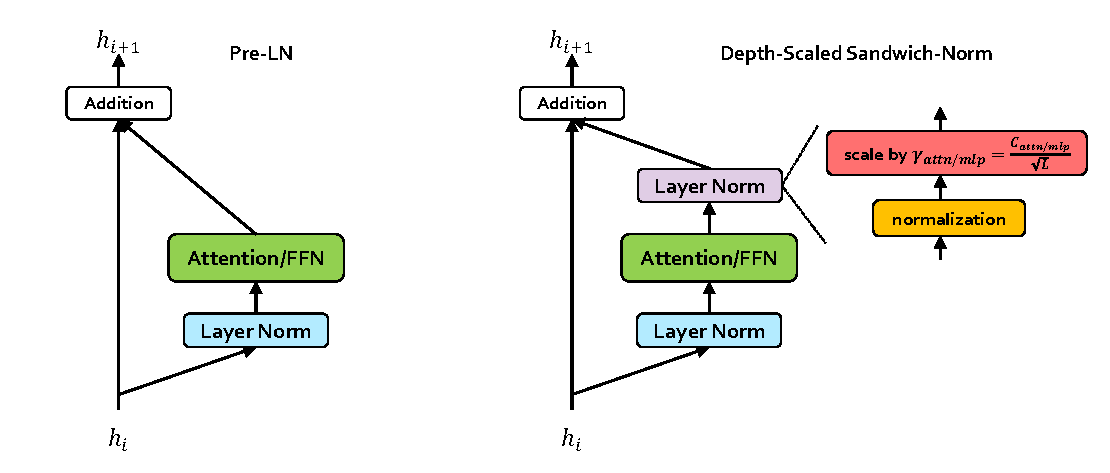
\includegraphics[width=0.8\textwidth]{fig/sandwich_arch.pdf}
    \caption{Pre-Layer Norm（Pre-LN）与 Depth-Scaled Sandwich-Norm（DSSN）结构对比。DSSN 在注意力和 FFN 模块前后都施加归一化层，而 Pre-LN 仅使用一层归一化。DSSN 还引入了深度缩放初始化，这是原始 sandwich norm 不具备的。}
    \label{fig:sandwich_arch}
\end{figure}

\subsection{模型初始化} \label{sec:tinyinit}

已有研究~\cite{nguyen2019transformers} 指出，模型初始化对训练稳定性和最终性能至关重要。
基于 Transformer 的 LLM 通常采用小尺度初始化~\cite{nguyen2019transformers}，即将权重按标准差 $\sqrt{\frac{2}{5d}}$ 的正态分布初始化，其中 $d$ 为隐藏维度。
另一个常见做法是按 $1/\sqrt{L}$~\cite{radford2019language} 缩放残差层权重初始化，其中 $L$ 为层数。

我们的发现是：同时结合模型深度与宽度进行缩放，即使用 $\sqrt{\frac{1}{2dL}}$，可以带来更快的 loss 收敛速度以及更好的下游任务表现。我们将该初始化称为 TinyInit。
我们推测 TinyInit 让模型各处参数尺度更一致，从而更利于优化与收敛。

研究~\cite{takase2024spikemore} 还表明，Embedding 层应采用与其他层不同的初始化策略。
具体来说，将 embedding 权重标准差保持在接近 1 的范围可能有助于训练稳定。
我们的实验表明，将其初始化为 0.5 可取得较好的模型性能。



\subsection{Tokenizer}\label{section:tokenizer}
Tokenizer 的设计会显著影响模型表现。理想词表需要同时兼顾领域覆盖（支持文本、数学、代码等多类任务）与编码效率（用更少 token 表示数据）。常见方法如 Byte-Pair Encoding（BPE）~\cite{shibata1999byte} 和 SentencePiece~\cite{kudo-richardson-2018-sentencepiece}，通常直接在全量训练数据上统计词频构建词表。但这种方式容易出现领域失衡：通用文本等高频领域主导词表，而数学、代码等数据量较小的专业领域表示不足。

\modelname~采用面向领域的词表策略。我们分别在通用中文、通用英文、代码和数学等多个领域独立做词频分析，构建领域词表后再合并去重，得到包含 153,376 个唯一 token 的统一词表。在保持整体压缩效率的同时，该方法实现了更均衡的跨领域表示。表~\ref{tab:vocab_distribution} 给出了各领域 token 分布。
\begin{table}[htbp]
\centering
\caption{\modelname 统一词表中的 token 分布。}
\label{tab:vocab_distribution}
\small
\begin{tabular}{lrr}
\toprule
\textbf{领域} & \textbf{Token 数量} & \textbf{占比 (\%)} \\
\midrule
English & 68,017 & 44.35 \\
Chinese & 41,053 & 26.77 \\
Other & 30,573 & 19.93 \\
Latin-based languages & 4,507 & 2.94 \\
Arabic & 2,755 & 1.80 \\
Korean & 2,733 & 1.78 \\
Mathematics & 2,139 & 1.39 \\
Japanese & 1,599 & 1.04 \\

\midrule
\textbf{Total} & \textbf{153,376} & \textbf{100.00} \\
\bottomrule
\end{tabular}
\end{table}
